\documentclass[11pt]{article}
\usepackage{UF_FRED_paper_style}
\usepackage{lipsum}
\onehalfspacing

\setlength{\droptitle}{-5em} %% Don't touch

\title{Trabajo Final Econometría 2022 -2}

% AUTHORS:
\author{Augusto Rico\\% Name author
    \href{mailto:arico@unal.edu.co}{\texttt{arico@unal.edu.co}} %% Email author 1 
\and Luis Ángel Palacio Bayuelo\\% Name author
    \href{mailto:lupalaciob@unal.edu.co}{\texttt{lupalaciob@unal.edu.co}} %% Email author 2
\and Diego Barreto\\% Name author
    \href{mailto:dibarretom@unal.edu.co}{\texttt{dibarretom@unal.edu.co}}%% Email author 3
    }

\date{\today}

\begin{document}

{\setstretch{.8} %% Don't touch
\maketitle


% %%%%%%%%%%%%%%%%%%%%%%%%%%%%%%%%%%%%%%%%%%%%%%%%%%%%%%%%%%
% %%%%%%%%%%%%%%%%%%%%%%%%%%%%%%%%%%%%%%%%%%%%%%%%%%%%%%%%%%
% BODY OF THE DOCUMENT
% %%%%%%%%%%%%%%%%%%%%%%%%%%%%%%%%%%%%%%%%%%%%%%%%%%%%%%%%%%
% %%%%%%%%%%%%%%%%%%%%%%%%%%%%%%%%%%%%%%%%%%%%%%%%%%%%%%%%%%


\section{Introducción}

Para los gobiernos es fundamental el bienestar económico, por lo que siempre buscan identificar variables que logren explicar el crecimiento continuo y sostenido de la producción interna, dado que identificando estas variables pueden evaluar cuan efectivas son las políticas publicas aplicadas en la economía con el fin de lograr un mayor bienestar social. Para este trabajo se considero que el impacto de estas políticas se encuentra en índices tales como son el de Progreso social (SPI), Innovación (IGI), GINI y Democrático, enfocándonos exclusivamente en la variación de producción interna, sin preocuparnos de factores tan importantes tales como efectos ambientales, comercio internacional, flujos migratorios, seguridad jurídica, asuntos de genero o raza, u otros, dado que esto podría complejizar de sobremanera el modelo.

Mediante esta investigación se busca saber si una identidad contable que a piori parece ser independiente de temas tan disimiles tales como progresos social, desigualdad, calidad democrática e innovación puede ser explicada positivamente por estos factores, logrando establecer alguna serie de políticas publicas beneficiosas para un bienestar tanto económico como social.

Para el modelo se analizara el PIB per Capíta ajustado a su poder adquisitivo, evaluado en la mayor cantidad de países posibles, principalmente restringido por la obtención de datos, frente las variables exógenas SPI, IGI, GINI y Democracia.





\section{Marco Teórico}

Como variable exógena se utilizara el producto interno bruto (PIB) per cápita a valores de paridad de poder adquisitivo (PPA) para evitar desviaciones en países donde el costo de vida sea elevado.


\subsection{Índice de progreso social (SPI)}

Aunque a piori puede que el PIB no tenga relación aparente con con el progreso social, dado que el PIB valora los bienes y servicios y no factores de calidad de vida. no obstante desde la creación de índices de bienestar social tales como el índice de desarrollo humano (IDH) se ha visto una alta correlación entre este y el logaritmo del PIB per cápita (Elistia, E., \& Syahzuni, B. A., 2018), lo que entra en concordancia con la teoría económica ortodoxa, donde Say (1821) argumenta que un mayor nivel de producción (PIB), implica un mayor nivel de demanda en la economía lo significa agentes consumidores con mayores niveles ingresos lo que se ve traducido en mayores niveles de utilidad (bienestar) ante un aumento de la producción total de la economía. 

Se prefirió utilizar el Índice de Progreso Social (SPI) frente el reconocido Índice de Desarrollo Humano (IDH) dado que dentro de la identidad de este índice se pondera con $1/3$ el PIB per capital (UNPD) por lo que puede determinar de sobremanera la correlación.


\subsection{Índice global de innovación (IGI)}



Sollow (1956), sugiere que parte del crecimiento económico a largo plazo, está relacionado con el uso de factores productivos (capital y trabajo) y el aumento del índice de productividad con el que se utilizan estos a través de la innovación. Existen dos conceptos claves para definir el papel que juega la innovación en el crecimiento económico. Por un lado, los aumentos en la eficiencia productiva debidos a la innovación y el desarrollo investigativo permite crear nuevos y mejores métodos de producción que en el mediano y largo plazo permitirán una mayor nivel de productividad y por ende un mayor margen de ganancias que puede ser reinvertido en nuevos procesos de producción que provoquen crecimiento económico; esta última parte hace referencia al segundo concepto “eficiencia dinámica”. Cuando se logra la eficiencia en los niveles de producción los países se hacen más atractivos para los inversionistas que va cambiando sus modos de actuar frente a la información.

Aunque para la teoría ortodoxa se conceptualiza que existe competencia perfecta, lo que implica que un desarrollo tecnológico pueda ser aprovechado por todos los países sin ningún tipo de restricción; si esto sucediera el desarrollo tecnológico sería homogéneo en todos los países y por ende no existiría correlación entre la innovación y la producción, no obstante es bien sabido que esto no se cumple en la economía empírica, siendo el principal determinante de esto la existencia de patentes que marcan la diferencia en el desarrollo tecnológico de la economía alrededor de los países, debido a esto se debe tener una relación positiva entre la innovación y el PIB.



\subsection{Coeficiente de GINI (Ingresos)}



La desigualdad es un factor que impacta aspectos económicos, políticos y sociales de forma negativa. Piketty (2014) sostiene que con una elevada desigualdad se tiende a promover la formación de burbujas en los precios de los activos, en la medida que el crecimiento en la demanda se impulsa más por el crédito al consumo que por los sueldos y salarios (como se citó en Alarco & Castillo, n.d.). Por otro lado, la desigualdad ocasiona  imperfecciones en los mercados capitales, lo que hace que las personas de bajo recursos no tengan las mismas posibilidades de educación, acceso a crédito y consumo que las persona de ingresos altos. Tomando en  cuenta lo anterior y analizando la bajo la perspectiva de Keynes, se tiene que la reducción de la propensión al consumo se traduce en una búsqueda de la eficiencia del capital, así como el aumento de la preferencia por la liquidez. En esta situación el dinero se desvía de la inversión al ahorro, lo que desemboca en desempleo, caída del consumo y distribución desigual de la renta. Esta asimetría informativa característica de los mercados financieros hace que los países con mayor desigualdad y alta pobreza absoluta infrautilizan su potencial productivo y de crecimiento respecto de los países con un menor número de pobres o con una distribución de renta más igualitaria. (Novales, s.f). 

Keynes afirma que es importante tener en cuenta el corto plazo de las economías, ya que los desplazamientos de esta demanda agregada influyen tanto en el crecimiento económico como en el nivel de precio, Asimismo, cuando el capitalismo es administrado bajo la propuesta clásica es incapaz de generar pleno empleo, lo que genera un distribución injusta de la riqueza y los ingresos limitando a la sociedad de oportunidades en el mercado, que es un factor importante para el crecimiento económico de un país. 



\subsection{Índice de democracia}

Para las corrientes institucionalistas, el sistema político es un importante determinante del crecimiento económico en el largo plazo;  Acemoglu, Johnson y Robinson. (2004) plantean que la explicación fundamental del crecimiento no es mas que las diferencias en las instituciones del país, ya que dado un entorno institucional adverso donde no se tenga una correcta separación de poderes el gobierno no tendrá incentivos en un crecimiento económico para poder mantener el poder, por lo que países con entornos democráticos y de control político activo van a lograr crecer mas en el largo plazo. Esto es evidenciado en el caso particular de Nigeria por Sala-i-Martin y Subramanian (2003). donde a pesar de grandes ingresos minero-energéticos el país no logra un crecimiento económico sostenido debido a un sistema institucional ineficiente que incentiva a grupos particulares a captar las rentas en detrimento del crecimiento económico a largo plazo, en contra parte con Botswana que como expone Auty (2008). con unas condiciones iniciales parecidas e incluso inferiores a las nigerianas gracias a la herencia británica de una democracia parlamentaria con estructuras de control político fuertes logro hoy tener una diferencia de mas de cinco mil dolares en el PIB per cápita con Nigeria país que sufrió constantes golpes de estados y regímenes poco democráticos.

Dado que este índice únicamente valida democracias liberales, en el modelo no se incluirá a países que no tengan como fin ser una democracia liberal, tales como son los estados socialistas, monarquías absolutistas o teocracias.


\section{Metodología }

\subsection{Especificación del modelo}
Las variables exógenas seleccionadas para desarrollar el modelo de regresión y explicar la variable endógena,  producto interno bruto (PIB) a valores de paridad de poder adquisitivo (PPA) per cápita, son: el progreso social, la innovación, la desigualdad entre ingresos y la democracia; recopilados a través del índice de Progreso Social (SPI) , Índice Global de Innovación (IGI), el coeficiente de GINI y el Índice de Democracia (Demc), respectivamente. 

$$ ln(GDP_{pc}^{ppp})_i = \beta_1 + \beta_2 SPI_i + \beta_3 IGI_i + \beta_4 GINI_i + \beta_5 Demc_i $$

Se utiliza un modelo log-lin, ya que resulta ́más conveniente y  ́útil conocer la incidencia
individual de cada variable sobre el PIB per cápita en forma porcentual, dado un aumento de un de una unidad de cada índice. Por lo expresado en el marco teórico, se espera que todos los índices  tenga una relación positiva con el crecimiento del (PIB) per cápita, salvo el índice GINI puesto que creemos que los países.

 
\subsection{Datos}

 Los datos recopilados y utilizados para la investigación son datos de corte transversal obtenidos de organismos económicos internacionales que se encargan de censar al grueso de los países a nivel global como el Fondo monetario internacional (FMI), la unidad de inteligencia de The economist y el Banco Mundial (BM);estas organizaciones manejan un amplio numero de relaciones con países de todo el mundo y expertos en la materia de análisis económico como las mediciones de variables para evaluar instituciones, innovación, bienestar social y medir ingresos entre países junto con su distribución. La definición de cada uno se encuentra a continuación:
 
\begin{itemize}
    \item El índice de progreso social (SPI): indicador que hace una valoración integral del bienestar de las personas en una sociedad, a partir de diferentes variables sociales, culturales y ambientales.
     \item El Índice Mundial de Innovación (IGI) para 2022 toma en cuenta las tendencias mundiales más recientes en materia de innovación en el contexto de la pandemia de COVID-19, la guerra y las perturbaciones que sufren la cadena de suministro y la energía. En el índice se actualizan las clasificaciones anuales relativas a los resultados de la innovación de 132 economías, destacando sus puntos fuertes y débiles en materia de innovación y las carencias de que adolecen en los datos sobre innovación.(IGI, n.d)
    \item El coeficiente Gini es el método más utilizado para medir la desigualdad salarial. Es una herramienta analítica que suele emplearse para medir la concentración de ingresos entre los habitantes de una región, en un periodo de tiempo determinado(BBVA, 2022)
    \item   El Índice de Democracia, publicado por The Economist Intelligence Unit está compuesto por cinco áreas de evaluación: el proceso electoral y su pluralismo, el funcionamiento del gobierno, la participación política, la cultura política y las libertades civiles. Los valores del índice se utilizan para ubicar a los países dentro de uno de los cuatro tipos de régimen:democracias plena, democracias defectuosas,regímenes híbridos y regímenes autoritarios.(FUNDESA, n.d)
\end{itemize}
 
 
 \subsection{Estimación}
El Método de Mínimos Cuadrados Ordinarios (MCO) será el utilizado para realizar la estimación del modelo de regresión. Este método se le atribuye al matemático Alemán Carl Friedrich Gauss. El procedimiento consiste en minimizar
la suma de los cuadrados de las distancias verticales entre los valores de los datos y los de la regresión estimada, es decir, minimizar la suma de los residuos al cuadrado, teniendo como residuo la diferencia entre los datos observados y los valores del modelo (n.d).

Dado $n$ pares de observaciones $Y_i$ y $X_i$, se pretende encontrar la función de regresión muestral (FRM)  $\hat{Y_i} = \hat{\beta_1} + \hat{\beta_2} X_i + \hat{u_i}$ que sea lo mas cercana posible a la $Y$ observada de la función de regresión poblacional (FRP) $Y_i = \beta_1 + \beta_2 X_i + u_i$. Con este fin, se adopta el siguiente criterio: seleccionar la FRM de modo que la suma de los residuos cuadrados $\sum u_i = \sum ( Y_i - \hat{Y_i})^2 $ sea la menor posible (Gujarati, 2010).

El método de MCO es uno de los más usados, ya que los estimadores obtenidos a través de este método las siguientes características que son muy deseables:
\begin{itemize}
    \item  Los estimadores de MCO se expresan únicamente en términos de las cantidades observables (es decir, muestras). Por consiguiente, se calculan con facilidad
    \item Pueden ser puntuales o por intervalos
    \item Una vez obtenidos los estimadores de MCO de los datos de la muestra, se obtiene sin problemas la línea de regresión muestral, la cual cuenta con la propiedades necesarias para la regresión.
\end{itemize}

\section{Estimación del Modelo}

\begin{table}[!htbp] \centering 
  \caption{} 
  \label{} 
\begin{tabular}{@{\extracolsep{5pt}}lc} 
\\[-1.8ex]\hline 
\hline \\[-1.8ex] 
 & \multicolumn{1}{c}{\textit{Dependent variable:}} \\ 
\cline{2-2} 
\\[-1.8ex] & GDP \\ 
\hline \\[-1.8ex] 
 SPI & 0.072$^{***}$ \\ 
  & p = 0.000 \\ 
  & \\ 
 GINI & 0.007 \\ 
  & p = 0.161 \\ 
  & \\ 
 IGI & 0.016$^{***}$ \\ 
  & p = 0.003 \\ 
  & \\ 
 DEMC & $-$0.009$^{***}$ \\ 
  & p = 0.002 \\ 
  & \\ 
 Constant & 4.292$^{***}$ \\ 
  & p = 0.000 \\ 
  & \\ 
\hline \\[-1.8ex] 
Observations & 145 \\ 
R$^{2}$ & 0.885 \\ 
Adjusted R$^{2}$ & 0.882 \\ 
Residual Std. Error & 0.410 (df = 140) \\ 
F Statistic & 269.631$^{***}$ (df = 4; 140) \\ 
\hline 
\hline \\[-1.8ex] 
\textit{Note:}  & \multicolumn{1}{r}{$^{*}$p$<$0.1; $^{**}$p$<$0.05; $^{***}$p$<$0.01} \\ 
\end{tabular} 
\end{table}

\begin{itemize}
    \item Por cada unidad que aumente el Índice de Progreso Social se estima que en promedio el PIB per cápita presente un aumento de 7,2 \%, manteniendo todo lo demás constante. 
    
    \item Por cada unidad que aumente la innovación se estima que en promedio el PIB per cápita aumente 1,6 \%, manteniendo todo lo demás constante.
    
    \item Por cada unidad que aumenta la desigual se estima que en promedio el Pib per cápita aumente 0,7 \% , manteniendo todo lo demás constante.
    
    \item Manteniendo todo lo demás constante por cada unidad que aumente la variable democracia se estima que en promedio el PIB per cápita disminuirá 0.9 \% 
\end{itemize}

Cabe aclarar que algunos valores de las variables, no son acordes con acordes con la teoría planteada, esto se puede deber a la existencia de algún error en los supuestos del modelo. No obstante, cualquier error existente se corregirá posteriormente.

\subsection{Pruebas de significancia Global e individual}

Como se puede ver en la tabla anterior, el F statistic que corresponde a la prueba de significancia global, muestra que el modelo es globalmente significativos a un nivel de significancia hasta de 0,01. 

En cuanto a la significancia individual, la variables SPI y IGI, son significativas a un nivel de sigmificancia de 0,1, mientras que la variable GINI es significativa a un alpha de 16\%.




\section{Verificación de supuestos}
\subsection{Correcta especificación}

Un error de especificación es el incumplimiento de cualquiera de los supuestos básicos del modelo lineal general. Esta expresión hace referencia al supuesto implícito de que las variables explicativas incluidas en el modelo son las verdaderamente relevantes en la explicación de $Y$. Entre los errores de especificación se encuentra la omisión de variables relevantes o la inclusión de variables irrelevantes. Si se estima el modelo con el primer problema los estimadores tienen a ser sesgados e inconsistentes, mientras que el segundo problema implica estimadores insesgados, pero se pierden grados de libertad injustificadamente. Para detectar si existe un error de especificación se usa el test de RESET (del inglés, Regression Epecification Error Test) de Ramsey. Este consiste  en realizar una regresión auxiliar del modelo original compuesta por la variables exógenas, más la potencia al cuadrado y al cubo de la variable endógena $Y_i$, expresada como

$$ ln(GDP_{pc}^{ppp})_i = \beta_1 + \beta_2 IGI_i + \beta_3 GINI_i + \beta_4 Demc_i $$

Donde la hipótesis nula viene dada por $H_0 : \gamma_1 = \gamma_2 = 0$ y representa la no existencia de un error de especificación en el modelo,mientras que la hipótesis alternativa $H_1 : \text{Al menos un } \gamma_1 \neq 0 \ \ \ i=1,2,... $  represente la existencia de un error de especificación. Para el modelo planteado en este trabajo, el p- value es de $0.3113$, resulto ser mayor que un nivel de significancia del 20 \% el cual se esta utilizando para la variable GINI,  debido a lo anterior no se rechaza la hipótesis nula, concluyendo que no existe un error de especificación.


\subsection{Cambio estructural}

El cambio estructural hace referencia a un cambio inesperado en una serie de tiempo. Esto puede hacer que se incurra en grandes errores predictivos y poca fiabilidad del modelo en general. Las consecuencias de estimar un modelo por MCO sin tener en cuenta un cambio en la estructura del modelo, representa que los estimadores van a ser sesgados e inconsistentes respecto al comportamiento de cada submuestra; insesgados debido a que el valor de los estimadores tiende a ser diferente del valor real de estos. Otra consecuencia del cambio estructural radica en que el tamaño de los residuos será mayor, esto involucra una SRC mayor, lo que implica un aumento en la varianza y por ende se pierde confiabilidad en el modelo. Al no tener en cuenta el cambio estructural el modelo es susceptible a presentar problemas de heteroscedasticidad o autocorrelación.

Dado que los datos usados para la estimación del modelo son datos de corte transversal, ninguna de las pruebas para detectar el cambio estructural resulta pertinente, debido a que por definición este problema solo se puede dar en datos de series de tiempo, es decir, se concluye por definición la no existencia de cambio estructural.

\subsection{Homocedasticidad}

El supuesto de homoscedasticidad implica que, condicionando en las variables explicativas la varianza del término de error no observado es constante, la violación a este supuesto es la heteroscedasticidad, donde la varianza del error es diferente para cada valor de $x$. Estimar un modelo con heteroscedasticidad implica tener estimadores MCO insesgados, además, como la $Var(u|X)$ ya no es constante, el estimador MCO ya no es MELI (Mejores Estimadores Lineales Insesgados) y el estimador MCO ya no es asintóticamente eficiente.

 Para detectar un problema de heteroscedasticidad, está la prueba propuesta por Breusch and Pagan (1979), que consiste en ajustar un modelo de regresión lineal con variables respuesta dadas por residuales del modelo original al cuadrado
 $$ \hat{u_i^2} = \gamma_1 + \gamma_2 x_i _2 + \gamma_3 x_i _3 + ..... + \gamma_k x_i _k $$
 
 y como covariables las variables del modelo original. Si se concluye que  $ \gamma_1 = \gamma_2 = \gamma_3 = \gamma_k = 0 $, significa que los residuales no son función de las covariables del modelo. El estadístico en esta prueba está dado por  $n * R^2$  y bajo la hipótesis nula verdadera, el estadístico tiene distribución $x_k^2$.
 
 Ddao que valor-P $3.019e-05$ es menor que el nivel de significancia trabajado, por lo tanto, hay evidencias para decir que no se cumple la homocedasticidad de los $ei$.

 Para corregir los problemas sobre los estimadores derivados de la heterocedasticidad se utiliza el método de mínimos cuadrados ponderados.
 
\subsection{Aucorrelación}

La autocorrelación se define como la perturbación de una observación cualquiera $u_i$ que está correlacionada con la perturbación de cualquier otra observación, es decir que las observaciones no son independientes. La estimación del modelo con violación a este supuesto implica fallas en los estimadores por MCO, puesto que estos ya no serán insesgados y de varianza mínima, por otra parte, la inferencia estadística que se obtiene de la matriz de varianzas y covarianzas no es correcta.

Para detectar este problema se usa la prueba Durbin - Watson, que detecta autocorrelación de primer orden. Despues de realizar la prueba el Durbin / Watson que arroja el paquete econométrico es de 1.8473, un numero muy cercano a 2, por lo cual se rechaza la existencia de autocorrelación de primer orden.

\subsection{Normalidad}

Uno de los supuestos básicos del modelo de regresión lineal clásico es el que los errores tengan distribución normal, si este supuesto no se cumple, no se  tiene la justificación teórica para la utilización de pruebas estadísticas que involucren a las distribuciones $t$, $F$ y $x^2$ .
 
La prueba Jarque-Bera (1987) permite evidenciar el supuesto de normalidad, consiste en obtener un valor estadístico que será contrastado con una distribución $x^2$ con dos grados de libertad, con base en la asimetría y la curtosis o apuntamiento de la gráfica de distribución de los residuos MCO. Al realizar esta prueba al modelo tratado en el presente texto, se encontró un p-value = 0.3603, por lo que se concluye normalidad para el modelo a un nivel de significancia incluso mayor al 20 \%, el cual se está trabajando para la variable GINI.

\subsection{Multicolinealidad}

El problema de multicolinealidad consiste en la existencia de relaciones lineales entre dos o más variables independientes del modelo. La multicolinealidad afecta la estimación de los parámetros que acompañan las variables exógenas, cuando existe este problema la matriz de varianzas y covarianzas del modelo no se puede estimar lo que implica una indeterminación de los estimadores.

Para identificar la existencia de un problema de multicolinealidad entre las variables, se debe calcular el índice de correlación entre todas las variables exógenas, dado el caso que alguno tenga un valor superior a 0,9 , se concluye un problema de multicolinealidad.

Los resultados de la estimación arrojan que a medida que aumenta la desigualdad y la democracia, el PIB per cápita (GDP) presenta un disminución, este resultado no concuerda con la teoría. Si embargo, el poco sentido lógico de estos estimadores se puede ver explicado por un problema de multicolinealidad entre las variables SPI-IGI, DEMC - SPI.

  \begin{figure}[H]
    \centering
    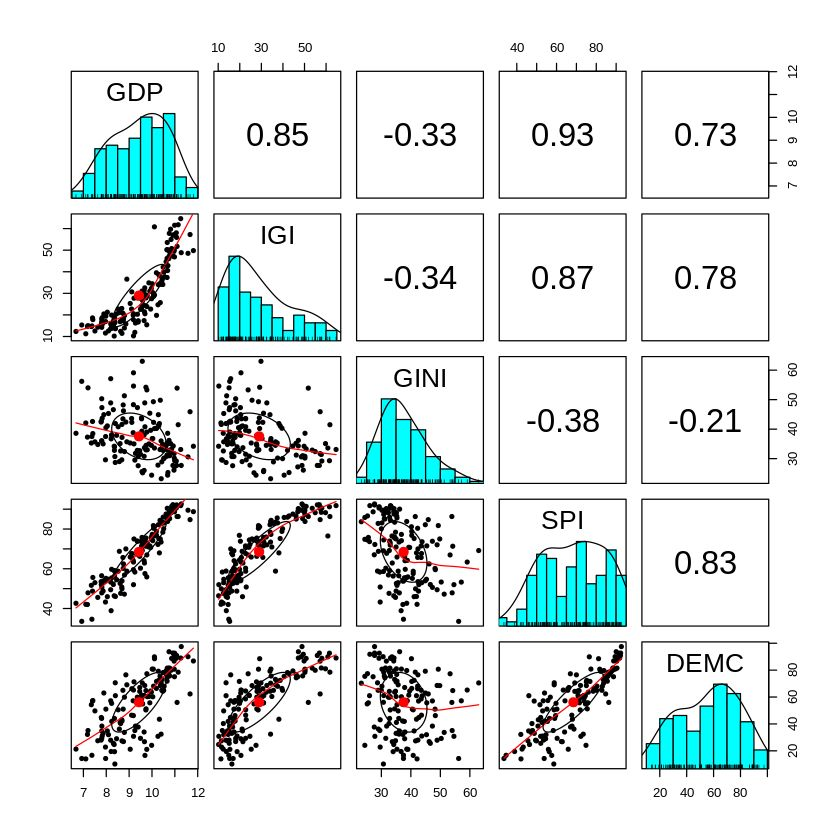
\includegraphics[scale=0.6]{WhatsApp Image 2022-10-30 at 5.53.10 PM.jpeg}
    \caption{}
    \label{fig:my_label}
\end{figure}

\section{Corrección a partir de la verificación de los supuestos}

Para solucionar el problema de multicolinealidad se optó por eliminar la variable SPI y se realizo la regresión por Mínimos Cuadrados Ponderados. En este caso, la especificación del modelo queda de la siguiente manera:

$$ln(GDP_{pc}^{ppp})_i = \beta_1 + \beta_2 IGI_i + \beta_3 GINI_i + \beta_4 Demc_i $$

\begin{table}[H] \centering 
  \caption{Comparacion modelos de estimacion PIB} 
  \label{} 
\begin{tabular}{@{\extracolsep{5pt}}lcc} 
\\[-1.8ex]\hline 
\hline \\[-1.8ex] 
 & \multicolumn{2}{c}{\textit{Dependent variable:}} \\ 
\cline{2-3} 
\\[-1.8ex] & \multicolumn{2}{c}{GDP} \\ 
\\[-1.8ex] & Original & Corregido\\ 
\hline \\[-1.8ex] 
 SPI & 0.072$^{***}$ &  \\ 
  & p = 0.000 &  \\ 
  & & \\ 
 DEMC & $-$0.009$^{***}$ & 0.009$^{**}$ \\ 
  & p = 0.002 & p = 0.019 \\ 
  & & \\ 
 GINI & 0.007 & $-$0.014$^{*}$ \\ 
  & p = 0.161 & p = 0.052 \\ 
  & & \\ 
 IGI & 0.016$^{***}$ & 0.056$^{***}$ \\ 
  & p = 0.003 & p = 0.000 \\ 
  & & \\ 
 Constant & 4.292$^{***}$ & 7.848$^{***}$ \\ 
  & p = 0.000 & p = 0.000 \\ 
  & & \\ 
\hline \\[-1.8ex] 
Observations & 145 & 145 \\ 
R$^{2}$ & 0.885 & 0.748 \\ 
Adjusted R$^{2}$ & 0.882 & 0.743 \\ 
Residual Std. Error & 0.410 (df = 140) & 0.100 (df = 141) \\ 
F Statistic & 269.631$^{***}$ (df = 4; 140) & 139.807$^{***}$ (df = 3; 141) \\ 
\hline 
\hline \\[-1.8ex] 
\textit{Note:}  & \multicolumn{2}{r}{$^{*}$p$<$0.1; $^{**}$p$<$0.05; $^{***}$p$<$0.01} \\ 
\end{tabular} 
\end{table} 

Al realizar la estimación omitiendo esta variable, se ve claramente que a medida que aumente el GINI el PIB per cápita presenta una disminución de 1,4 \% y a medida que aumenta la Índice de Democracia el PIB per cápita presenta un aumento 0,09 \%, lo que claramente concuerda con el marco teórico. Por otro lado, la prueba de Breusch-Pagan arrojo un p-value = 0.6918, lo que elimina cualquier problema de heteroscedasticidad a cualquier nivel de alpha común.

\section{Resultados}

 \subsection{Interpretación final de los parámetros estimados}

 Luego de realizar los ajustes pertinentes al modelo original se obtiene como resultado el modelo presentado en el cuadro 2. Estas estimaciones de los parámetros que acompañan a las variables involucradas en el modelo corregido a diferencia del los valores de los parámetros anteriores son acordes al marco teórico y presentan la tendecia esperada

\begin{itemize}
    \item Por cada unidad que aumente el Índice Global de Innovación manteniendo las demás variables constantes, se estima que en promedio el PIB Per cápita aumentará un 5,6 \%.

    \item Por cada unidad que aumente el GINI manteniendo las demás variables constantes, se estima que en promedio el PIB per cápita disminuirá en un 1,4 \%.

    \item Por cada unidad que aumente el Índice de Democracia manteniendo todo lo demás constante, se estima que en promedio el PIB per cápita aumentará un 0,9 \%.

    
    \end{itemize}
 

\subsection{Prueba de hipótesis individual y global}

Como se puede ver en la tabla anterior, el F statistic que corresponde a la prueba de significancia global, muestra que el modelo es globalmente significativo a un nivel de significancia hasta de 0,01. 

En cuanto a la significancia individual, todos las variables exógenas son significativas a un alpha de 0,1.


\subsection{Interpretación de intervalos de confianza}

Los intervalos de confianza para los componentes de $\beta$ están dados por:
$$ \hat{\beta_i} \pm t_{n-p-1} (L\alpha/2) \sqrt{\hat{V} (\hat{\beta})_{ii}}$$
\begin{itemize}
    \item Donde $\hat{\beta_i}$ es la $i$ - ésima entrada de \hat{\beta}
    \item $t _{ n - p-1} (\alpha / 2) $ es cuantil superior $\alpha / 2$ de una distribución $t _{ n - p-1}$
    \item $\hat{V} (\hat{\beta})_{ii}$ es el i-ésimo elemento de la diagonal
\end{itemize}

\begin{table}[ht]
\centering
\begin{tabular}{rrrr}
  \hline
 & Lim\_inf & Beta & Lim\_sup \\ 
  \hline
DEMC & 0.007 & 0.009 & 0.010 \\ 
  GINI & -0.012 & -0.014 & -0.016 \\ 
  IGI & 0.047 & 0.056 & 0.065 \\ 
   \hline
\end{tabular}
\end{table}

\begin{itemize}
    \item   El intervalo para la variable Índice de Democracia con un nivel de confianza de 90 \% para $\beta_2$ es ( 0.007, 0.010 ). Podemos estar interesados en decir que el modelo debe incluir el valor de la democracia en la explicación de PIB pér cápita. Este intervalo esta conformado por valores positivos, lo que nos lleva sostener que el efecto de DEMC sobre el PIB es positivo, con una significancia  $\alpha =0.01$ .

    \item   El intervalo para la exógena GINI con un nivel de confianza de 90 \% para $\beta_3$ es ( -0.012, -0.016 ). Podemos estar interesados en decir que el modelo debe incluir el valor de la desigualdad en la explicación de PIB pér cápita. Este intervalo esta conformado por valores negativos, lo que nos lleva sostener que el aumento de la desigualdad sobre el PIB pér cápita implica un efecto negativo, con una significancia  $\alpha =0.01$ .

    \item  El intervalo para el Índice Global de Innovación con un nivel de confianza de 90 \% para $\beta_4$ es (0.047, 0.065). Podemos estar interesados en decir que el modelo debe incluir el valor de la desigualdad en la explicación de PIB pér cápita. Este intervalo esta conformado por valores positivos, lo que nos lleva sostener que el aumento del IGI genera un efecto positivo sobre el PIB pér cápita , con una significancia  $\alpha =0.01$  .
    
\end{itemize}



\subsection{Comparación entre el PIB y el PIB estimado}

  \begin{figure}[H]
    \centering
    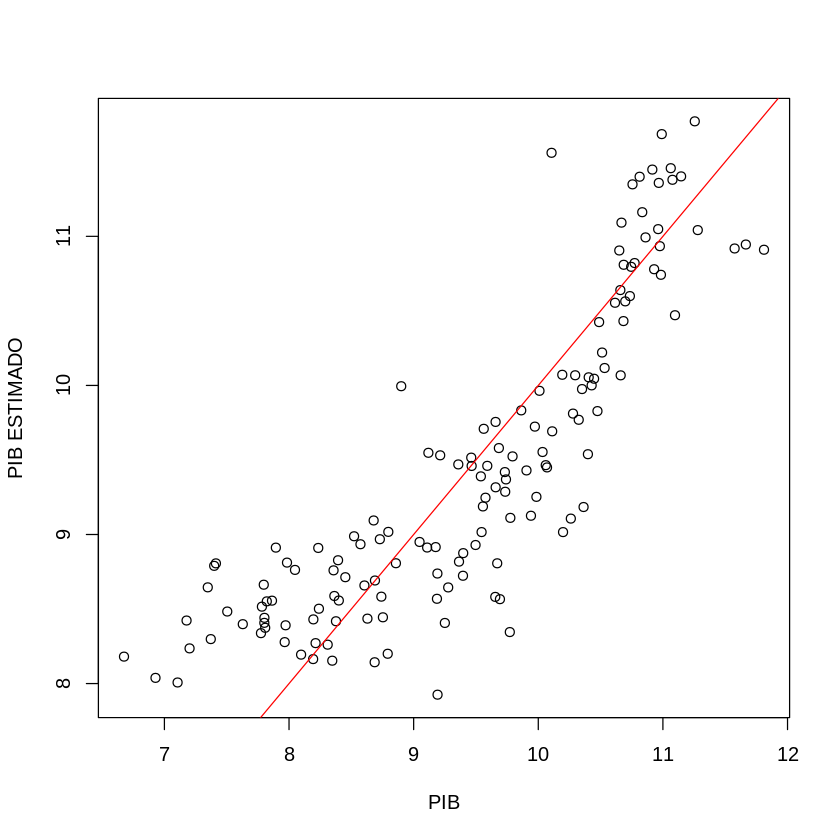
\includegraphics[scale=0.6]{download.png}
    \caption{}
    \label{fig:my_label}
\end{figure}

En la gráfica se puede observar que el modelo en términos generales se ajusta bien a los datos, ya que diferencias entre los valores observados y los valores de predicción del modelo no son tan grandes, por lo que no hay niveles altos de sesgo. Además el coeficiente R2 para el modelo corregido es de 0.748, es decir que las variables exógenas están explicando en un 74 \% la variabilidad de la endógena.

 \section{Pronóstico}
 
\begin{table}[H]
\centering
\begin{tabular}{rllrr}
  \hline\\
 QUANTILE & Country & GDP & GDP\_ESTIM \\ 
  \hline\\
 Q1 & Papua New Guinea & 8.40 & 8.56 \\ 
 Median & Ukraine & 9.56 & 9.71 \\ 
 Q3 & Croatia & 10.43 & 10.00 \\ 
  & Mean & 9.43 & 9.43 \\ 
   \hline
\end{tabular}
\end{table}

Papua New Guine, Ucrania, Croacia corresponden a primer cuartil, mediada, tercer cuartil, respectivamente. Además estos valores estimados son cercanos a los verdaderos por lo que podemos concluir que le modelo presenta un buen estimador.

 \section{Conclusiones} 

 i) Encontramos que usando variables que miden el bienestar social como la distribución de la riqueza (GINI), el índice de innovación (IGI) y y el índice de medida de democracia son relevantes a la hora de analizar una posible medida de desarrollo que permita estimular un crecimiento económico tanto a corto como largo plazo, esto basado en las teorías de desarrollo que apelan a favor de las instituciones nacionales que recaen sobre la democracias, una distribución mas equitativa de los ingresos entre los habitantes del país y por supuesto 
 
 ii) También concluimos que la estimación de mínimos cuadrados ordinarios no fue el mejor estimador posible para datos de corte trasversal y analizando las relaciones existentes entre variables endógenas del modelo es encontró una fuerte relación del índice de progreso social con las demás variables, para evitar errores de multicolinealidad se optó por eliminarla del modelo y producto de ello se nos permitió ver la relevancia y su importancia dentro del modelo, así como su cambio en el indicador GINI, a partir de la estimación del nuevo modelo se puede concluir que la teoría concuerda con las interpretaciones presentadas. 

 Al finalizar el modelo se concluye, en primer lugar, que las variables exógenas analizadas (IGI, DEMC), guardan una relación positiva con en el comportamiento del PIB per cápita de la muestra en la que se incluyeron diferentes países de los cinco continentes, mientras que la variables GINI, presenta un relación negativa. El modelo ofrece un panorama general del comportamiento mundial en cuanto a indicadores macroeconómicos que cobran importancia en la medida en que estos están abiertamente relacionados con temas de tipo socioeconómico.

 \section{Referencias}
 
Vela Peón, F. (2010). Normalidad de los errores. Universidad Autónoma Metropolitana.\\ https://mregresion.files.wordpress.com/2011/10/normalidad.pdf

Miranda, J. (2017, 8 agosto). Autocorrelación. Todo econometría. \\
https://todoeconometria.wordpress.com/2017/08/08/autocorrelacion/

Hernández, F. (2020, 30 octubre). 11 Pruebas de Homocedasticidad | Modelos de Regresión con R. Modelos de regresión en R. https://fhernanb.github.io/libroregresion/homo.html

Moreno, P., Rodriguez, J. M., & Soberon, A. (s. f.). Econometría I | Tema 6: Heterocedasticidad. Econometría I. \\ https://ocw.unican.es/pluginfile.php/1127/course/section/1352

Salmerón, R. (s. f.). Multicolinealidad. Multicolinealidad, Universidad de Granada.\\ https://www.ugr.es/~romansg/material/WebEco/02-Eco/Teoria/tema4.pdf

 Alarco, G., & Castillo, C. (n.d.). Índice de desigualdad y crecimiento económico en América Latina. Universidad Del Pacífico (Perú). https://www.scielo.org.mx/scielo.php?script=sci_arttext&pid=S0185-16672020000400106
 
 Coeficiente de Gini, el detector de la desigualdad salarial. (2022, September 30). BBVA NOTICIAS. https://www.bbva.com/es/coeficiente-gini-detector-la-desigualdad-salarial/
 
 FUNDESA - Índice de Democracia. (n.d.). Retrieved October 30, 2022, from https://www.fundesa.org.gt/
 indices-y-evaluaciones-de-pais/indices-internacionales/indice-de-democracia
 
 Índice Mundial de Innovación. (n.d.). Retrieved October 30, 2022, from https://www.wipo.int/global
 innovation_index/es/
 
 Método de los Mínimos Cuadrados Ordinarios. (n.d.). http://catarina.udlap.mx/u_dl_a/tales/documentos/lad/mercado_g_ja/apendiceC.pdf.
 
 Novales, A. (n.d.). CRECIMIENTO ECONÓMICO, DESIGUALDAD Y POBREZA. Portal Académico. https://www.boe.es/biblioteca_juridica/anuarios_derecho/abrir_pdf.php?id=ANU-M-2011-10041900432

Elistia, E., & Syahzuni, B. A. (2018). The correlation of the human development index (HDI) towards economic growth (GDP per capita) in 10 ASEAN member countries. Jhss (journal of humanities and social studies), 2(2), 40-46.

Acemoglu, D., Johnson, S., & Robinson, J. A. (2004). Institutions as a fundamental cause of long-run growth. Handbook of economic growth, 1, 385-472.

Auty, R. (2008). Political economy of African mineral revenue deployment: Angola, Botswana, Nigeria and Zambia compared. WP, 28, 2008

Sala-i-Martin, X., & Subramanian, A. (2003). Addressing the curse of natural resources: an illustration from Nigeria. NBER working paper, 9804.

 

\newpage

% %%%%%%%%%%%%%%%%%%%%%%%%%%%%%%%%%%%%%%%%%%%%%%%%%%%%%%%%%%
% %%%%%%%%%%%%%%%%%%%%%%%%%%%%%%%%%%%%%%%%%%%%%%%%%%%%%%%%%%
% REFERENCES SECTION
% %%%%%%%%%%%%%%%%%%%%%%%%%%%%%%%%%%%%%%%%%%%%%%%%%%%%%%%%%%
% %%%%%%%%%%%%%%%%%%%%%%%%%%%%%%%%%%%%%%%%%%%%%%%%%%%%%%%%%%
\medskip


\newpage

\end{document}